

\chapter{Informaci\'on de campo.}

\section{Recorrido de campo}

El recorrido de campo se realiz\'o entre los d\'ias 22 y 24 de noviembre de 2017. La zona recorrida se tuvo como prop\'osito divisar y en lo posible muestrear aquellos lugares que mostraron menor factor de seguridad en las pruebas preliminares y apreciar el estado de las unidades geol\'ogicas que muestra la cartograf\'ia estudiada.

En campo se pudo corroborar la consistencia de la unidad geol\'ogica predominante \(\mathsf{K_{saau}}\) (limolita), dicho material se pudo apreciar en todo el recorrido, con leve variaci\'on en su grado de meteorizaci\'on, principalmente en zonas de abundante vegetaci\'on. La morfolog\'ia abrupta de las laderas permiti\'o apreciar abundantes cicatrices de anteriores desprendimientos de material, principalmente en sectores de alta pendiente y en el trazado de la carretera que une las poblaciones de La Mansa hacia Quibd\'o en el departamento de Choc\'o.

\begin{figure}[H]
  \centering
  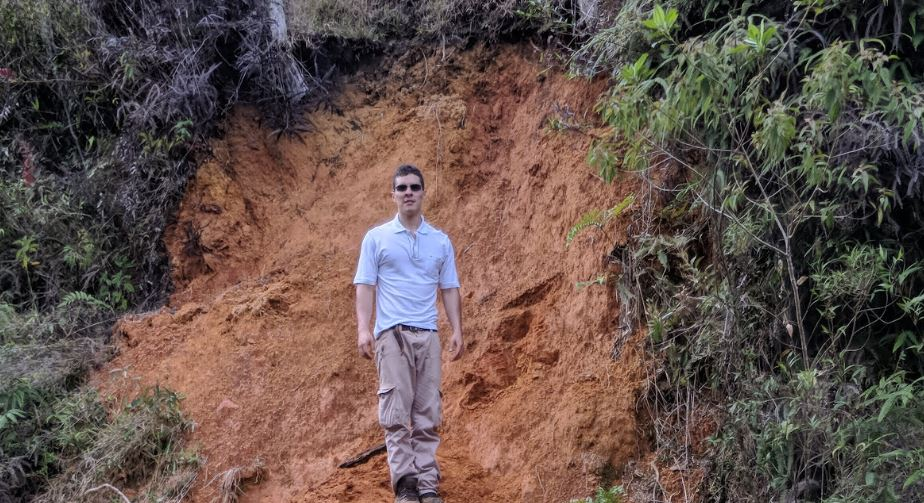
\includegraphics[scale=0.75]{img/estacion10.jpg}
  \caption{Lugar de toma de muestra de la estaci\'on 1. Aqu\'i se descartaron las zonas con material inalterado para toma de muestra en tubos PVC. Dichas muestras se tomaron donde se pod\'ia observar que el suelo conservaba su estructura original. }
  \label{fig:afloramiento}
\end{figure}

Se trabaj\'o en dos estaciones, en cada una de las cuales se realiz\'o la respectiva toma de muestra, siendo la primera de ellas la que m\'as informaci\'on proveer\'ia en los posteriores ensayos de laboratorio. Para la toma de muestra se tuvo la precauci\'on de seleccionar un lugar que no presentase retrabajamiento del material y en el cual se pudiese observar que el suelo presentase unas condiciones representativas del material observado durante los recorridos realizados.
Las muestras tomadas en la segunda estaci\'on se tomaron a una profundidad m\'a s somera (no mayor al metro) con la intenci\'on de posteriormente obtener los par\'a metros de resistencia de instancias m\'a s avanzadas de meteorizaci\'on de la limonita. Esto dado que las cicatrices de movimientos en masa observadas aparentaban que aquellos eventos ocurridos se dieron hace un tiempo considerable (a juzgar por el crecimiento nueva cobertura vegetal) no contaron con profundidades considerables de su respectiva superficie de falla. Asimismo, el testimonio obtenido de una habitante del lugar, corrobora que no son frecuentes movimientos que comprendan altos vol\'umenes de material, habiendo ocurrido el \'ultimo aproximadamente cinco a\~nos antes de la visita de campo.

La estaci\'on primera se realiz\'o en las coordenadas \(5.8712778, -76.0848778\), mientras que la estaci\'on segunda se realiz\'o en las las coordenadas \(5.8612472,-76.0927833\).
A continuaci\'on se detalla la informac\'on de ambas estaciones.

\textbf{Muestras recolectadas}

De la estaci\'on 1 se obtuvo:
\begin{itemize}
  \item muestra al interior de cuatro tubos PVC de \(2"\) de di\'ametro y apr\'oximadamente \(15\,\text{cm}\) de alto;
  \item un bloque de muestra inalterada  de apr\'oximadamente \(40 \times 40 \times 30\)[cm\(^3\)];
  \item una masa de \(200\,\text{g}\) de muestra alterada.
\end{itemize}

De la estaci\'on 2 se obtuvo:
\begin{itemize}
  \item Muestra al interior de 3 tubos PVC de \(2"\) de di\'ametro y apr\'oximadamente \(15\,\text{cm}\) de alto.
\end{itemize}

\begin{figure}[H]+
\centering
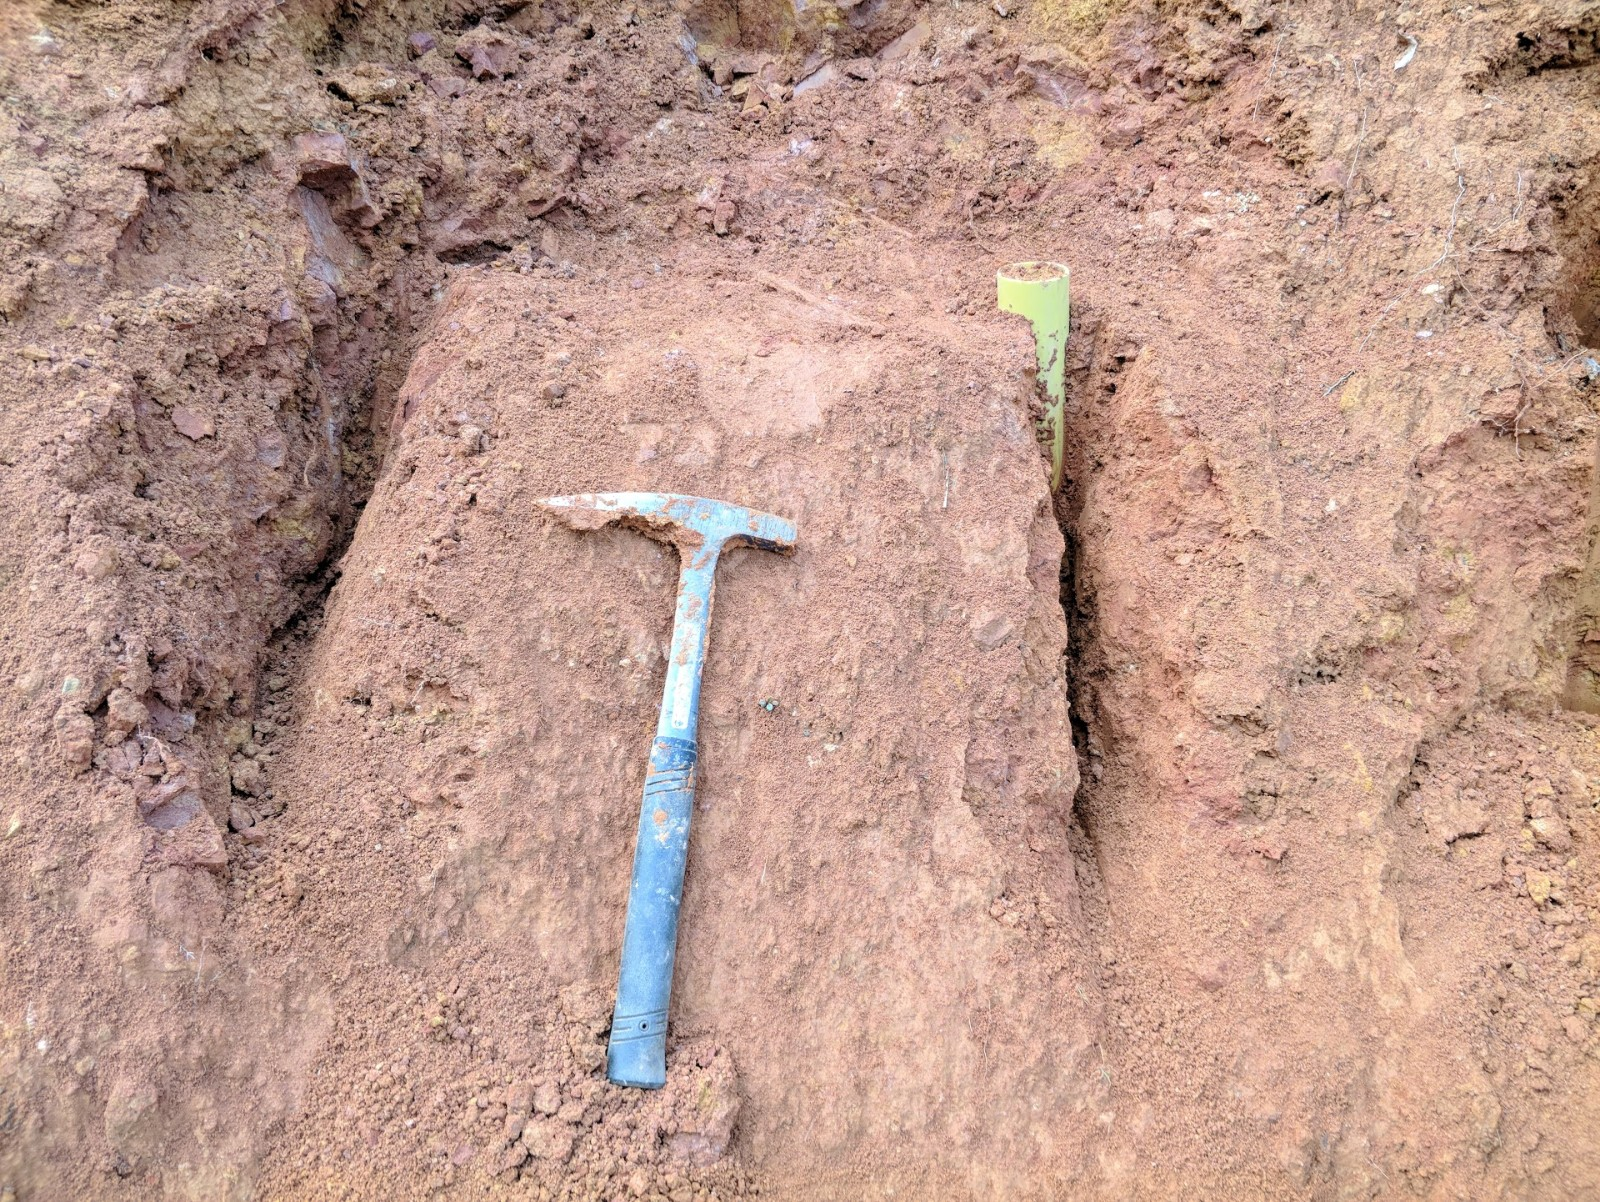
\includegraphics[scale=0.20]{img/estacion11.jpg}
\caption{Momento de toma de muestra inalterada, se tom\'o muestra en bloque as\'i como muestra confinada en tubos PCV de dos pulgadas.}
\label{fig:toma-bloque}
\end{figure}

\section{Ensayos de laboratorio.}

Las muestras recolectadas fueron analizadas en el laboratorio de suelos de a Universidad Nacional de Colombia, sede Medell\'in.
Como resultado de los ensayos se pudo determinar una humedad natural del \(21\,\%\).
La gravedad espec\'ifica de los s\'olidos, seg\'un el procedimiento descrito en la norma ASTM C-127 fue de \(2.53\).
Con estos valores se procedi\'o a realizar los ensayos de corte directo seg\'un la norma ASTM D-380. Se decidi\'o realizar los ensayos bajo condiciones de suelo saturado, con el prop\'osito de obtener par\'ametros correspondientes a eventos de alta precipitaci\'on que puedan presentarse en la zona de trabajo.

Los par\'ametros de resistencia obtenidos son \'angulo de fricci\'on interna saturada de \(40\,^\circ\) y cohesi\'on de \(29\,\text{kPa}\). Las hojas de c\'alculo de estos ensayos se adjuntan como anexos al presente trabajo.
En la tabla \ref{table:line}  se exponen los valores de resistencia al corte obtenido por cada muestra  y la carga aplicada. Y en la figura \ref{fig:line} se grafican los puntos maximos de resistencia de cada muestra



\begin{figure}[H]
\centering
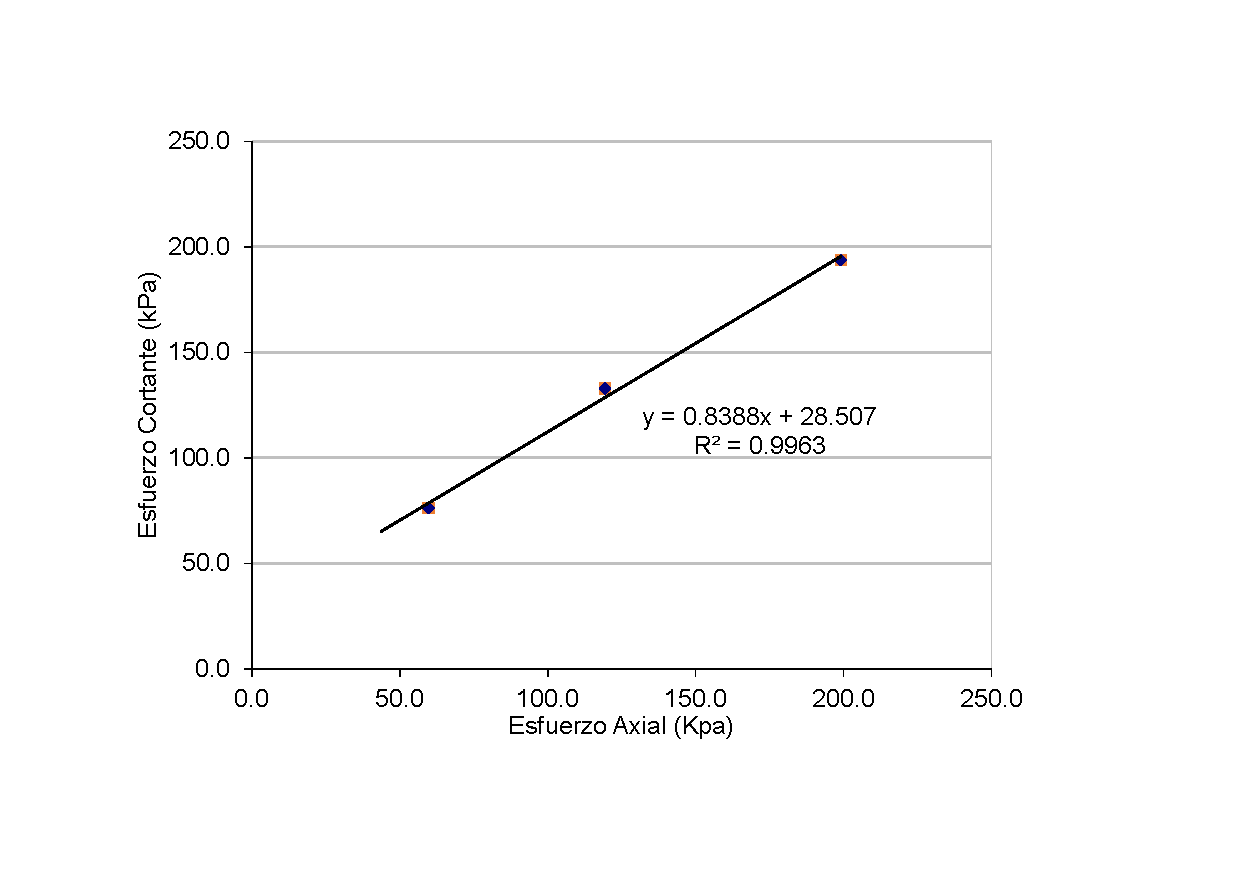
\includegraphics[trim={0 1.5cm 0 1.5cm},clip,scale=0.8]{img/line.pdf}
\caption{Estimaci\'on de par\'ametros de resistencia al corte basados en los datos de las muestras analizadas en la estaci\'on 1.}
\label{fig:line}
\end{figure}

\begin{table}[H]
\centering
\caption{Resultado de esfuerzo cortante para cada etapa de carga (Esfuerzo Axial) obtenida para las 3 muestras recolectadas en la estaci\'on 1.}
\begin{tabular}{|lc|cc}
\hline
\multicolumn{1}{|l|}{Muestra}                                                               & 1                       & \multicolumn{1}{c|}{2}     & \multicolumn{1}{c|}{3}     \\ \hline
\multicolumn{1}{|l|}{\begin{tabular}[c]{@{}l@{}}Esfuerzo Cortante\\   $\left( kPa \right) $\end{tabular}} & 76.2                    & \multicolumn{1}{c|}{132.8} & \multicolumn{1}{c|}{194}   \\ \hline
\multicolumn{1}{|l|}{Esfuerzo Axial $\left( kPa \right) $}                                                & 59.7                    & \multicolumn{1}{c|}{119.4} & \multicolumn{1}{c|}{199.1} \\ \hline
Angulo de Fricci\'on $  $                                                                      & \multicolumn{1}{l|}{40} & \multicolumn{1}{l}{}       & \multicolumn{1}{l}{}       \\ \cline{1-2}
Cohesi\'on $\left( kPa \right) $                                                                            & \multicolumn{1}{l|}{29} & \multicolumn{1}{l}{}       & \multicolumn{1}{l}{}       \\ \cline{1-2}
\end{tabular}
\label{table:line}
\end{table}





\paragraph{Scoops3D.}
Tomando los resultados de laboratorio expuestos anteriormente se procedi\'o a ingresar los valores correspondientes al \'angulo de fricci\'on, cohesi\'on y gravedad espec\'ifica en Scoops3D. Se mantuvo la configuraci\'on de caja de b\'usqueda descrita en la figura \ref{fig:test}.

\begin{figure}[H]
\centering
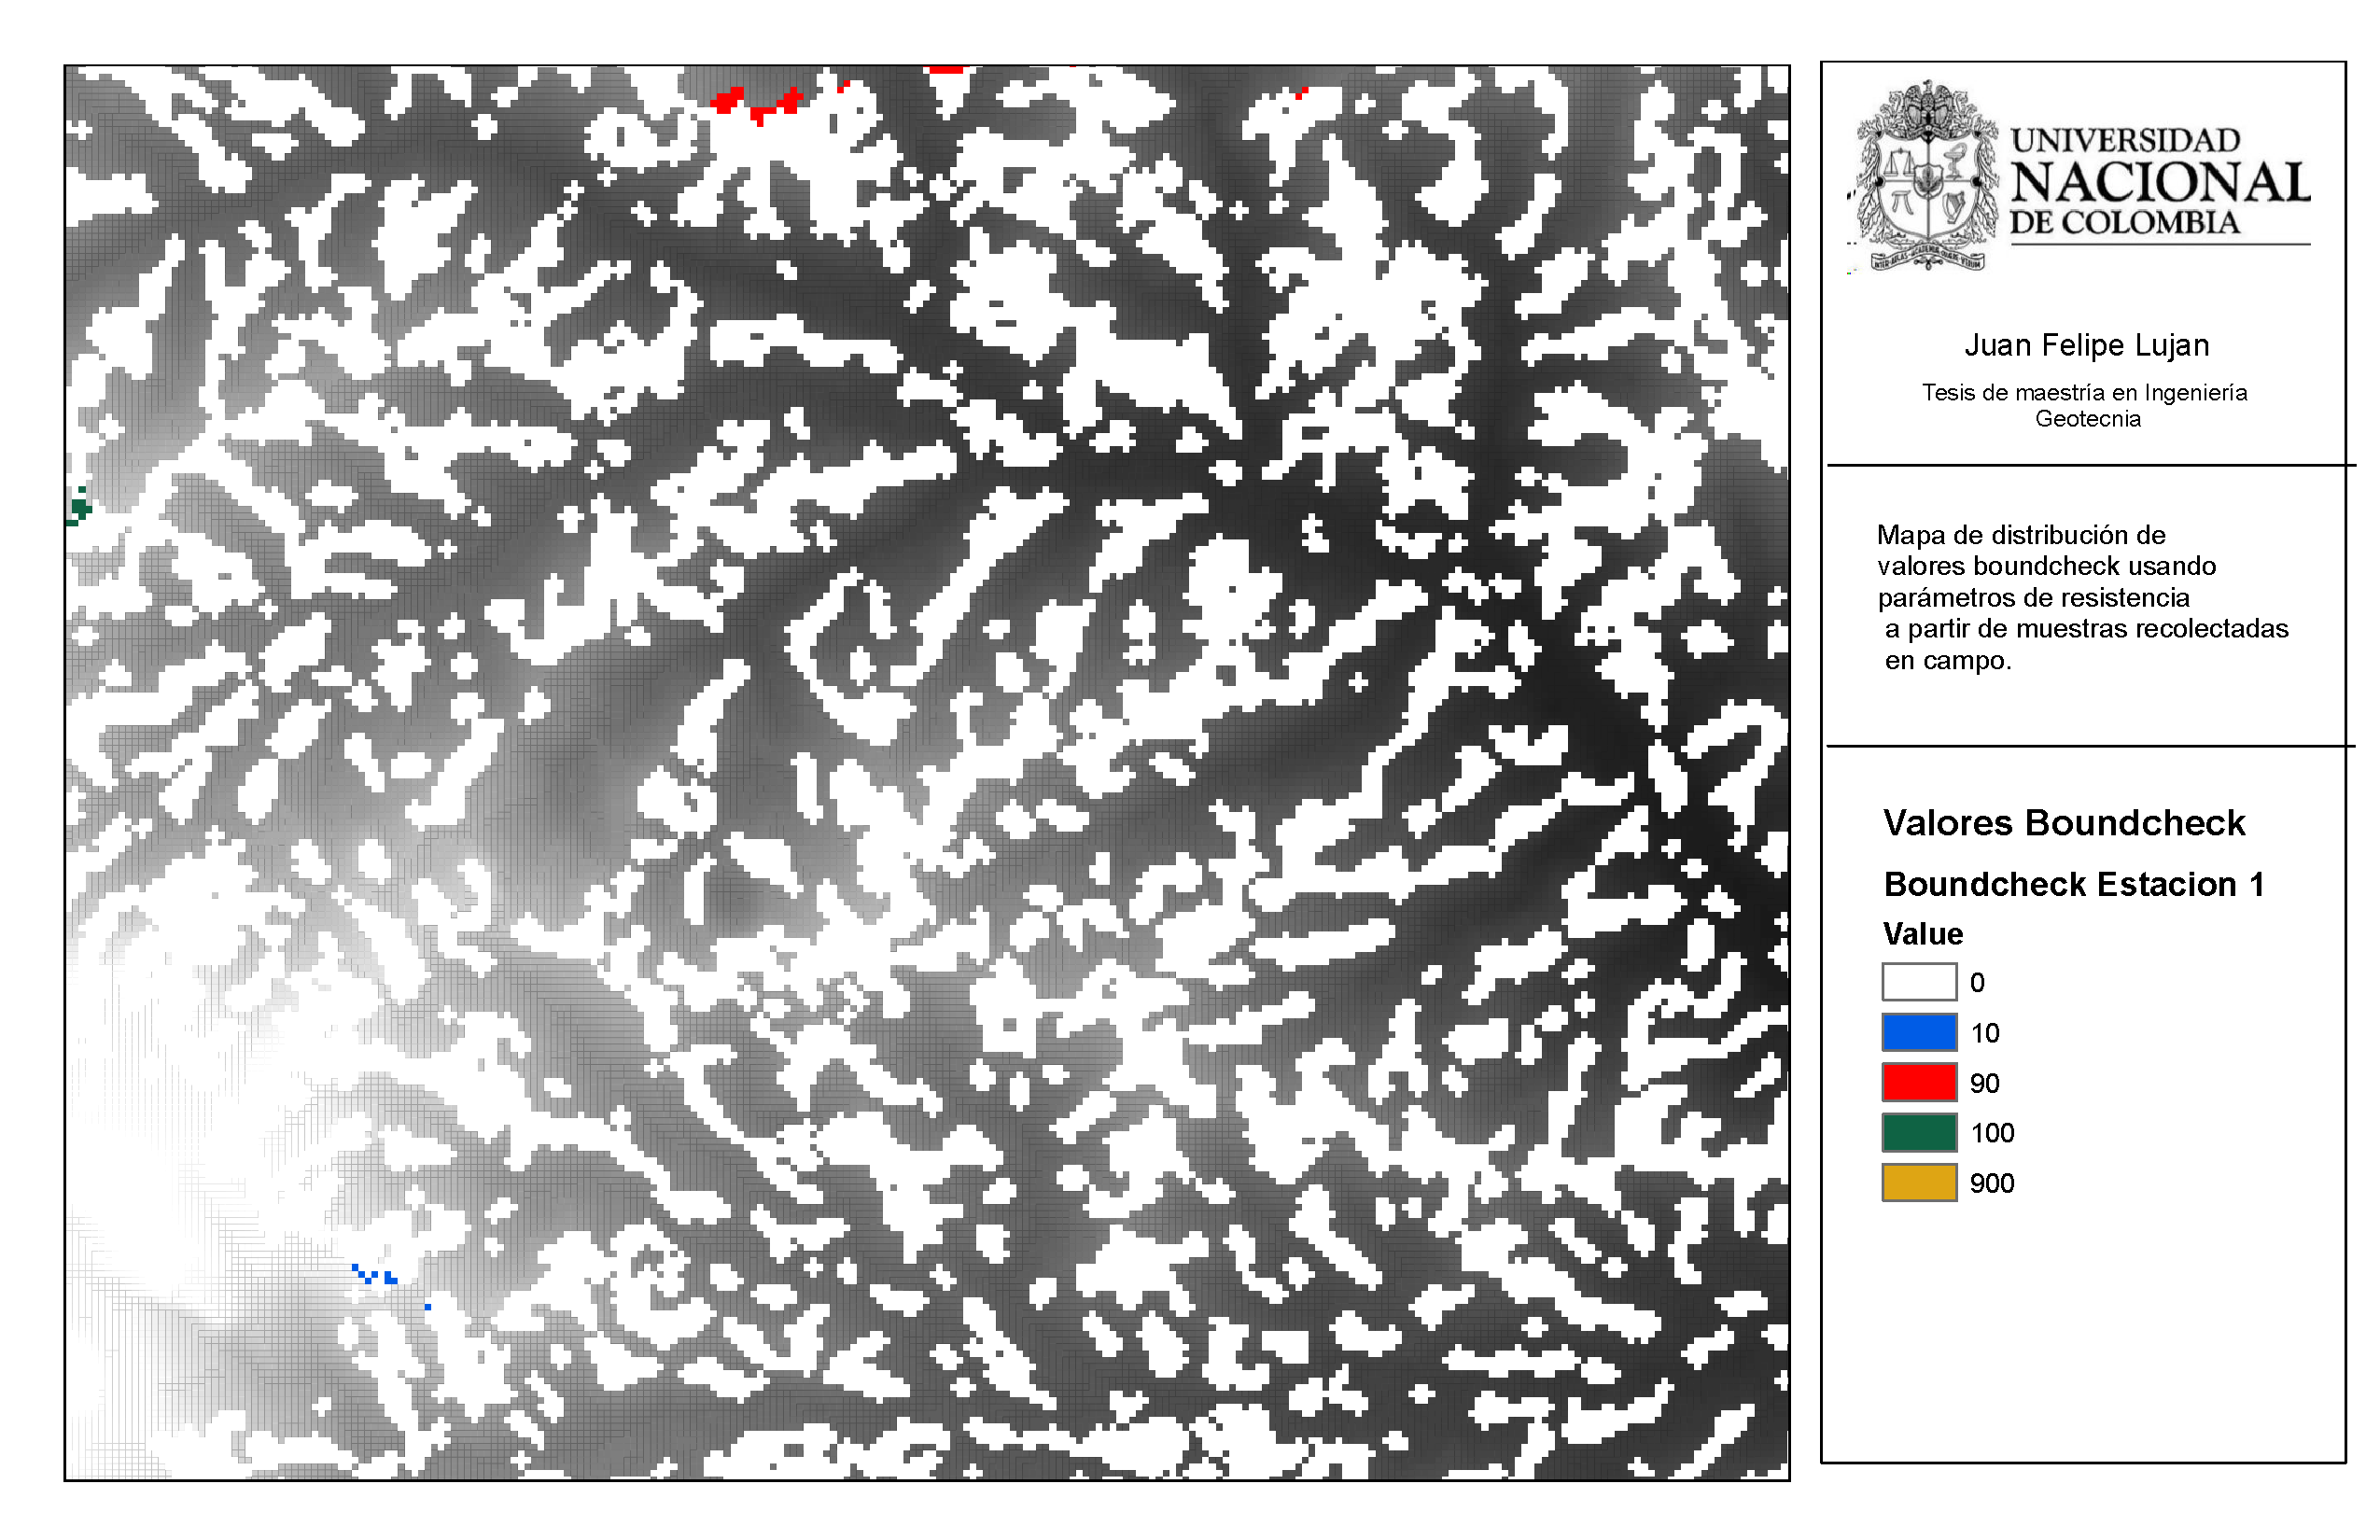
\includegraphics[scale=0.3]{img/boundcheckCampo.pdf}
\caption{Control de calidad a la corrida de Scoops3D con datos de campo por media del an\'alisis del archivo de salida Boundcheck. Fuente: Elaboraci\'on propia.}
\label{fig:dem usado}
\end{figure}

Se puede apreciar en el archivo de salida \textsf{boundcheck} que la caja de busqueda propuesta en las pruebas preliminares es aplicable los datos obtenidos de las muestras recolectadas en campo. Dicho comportamento era esperado debido a la abundancia de pendientes pronunciadas en esta zona del municipio de Ciudad Bolivar.

Los p\'ixeles marcados con color azul en el sector suroccidental de la zona de trabajo indican que la extension de la caja de busqueda hacia el extremo sur fue una limitante para aplicar el m\'etodo bishop (centro de la superficie de falla por fuera de la caja de busqueda, en direccion sur) lo mismo ocurre con los pixeles marcados de color rojo hacia el extremo norte de la zona de trabajo (centro de la superficie de falla por fuera de la caja de busqueda, en direccion norte)

Sin embargo, dado que la cuenta de p\'ixeles donde se presenta dicho comportamiento es de 89 sobre un total de 28057, se puede decir que la caja de b\'usqueda usada es aplicable en un 99.996\% a la zona de trabajo.
Para aumentar la cobertura ser\'ia necesario realizar pruebas en equipos de computo con mayores capacidades de computo a las descritas en el cap\'itulo 5.


\begin{figure}[H]
\centering
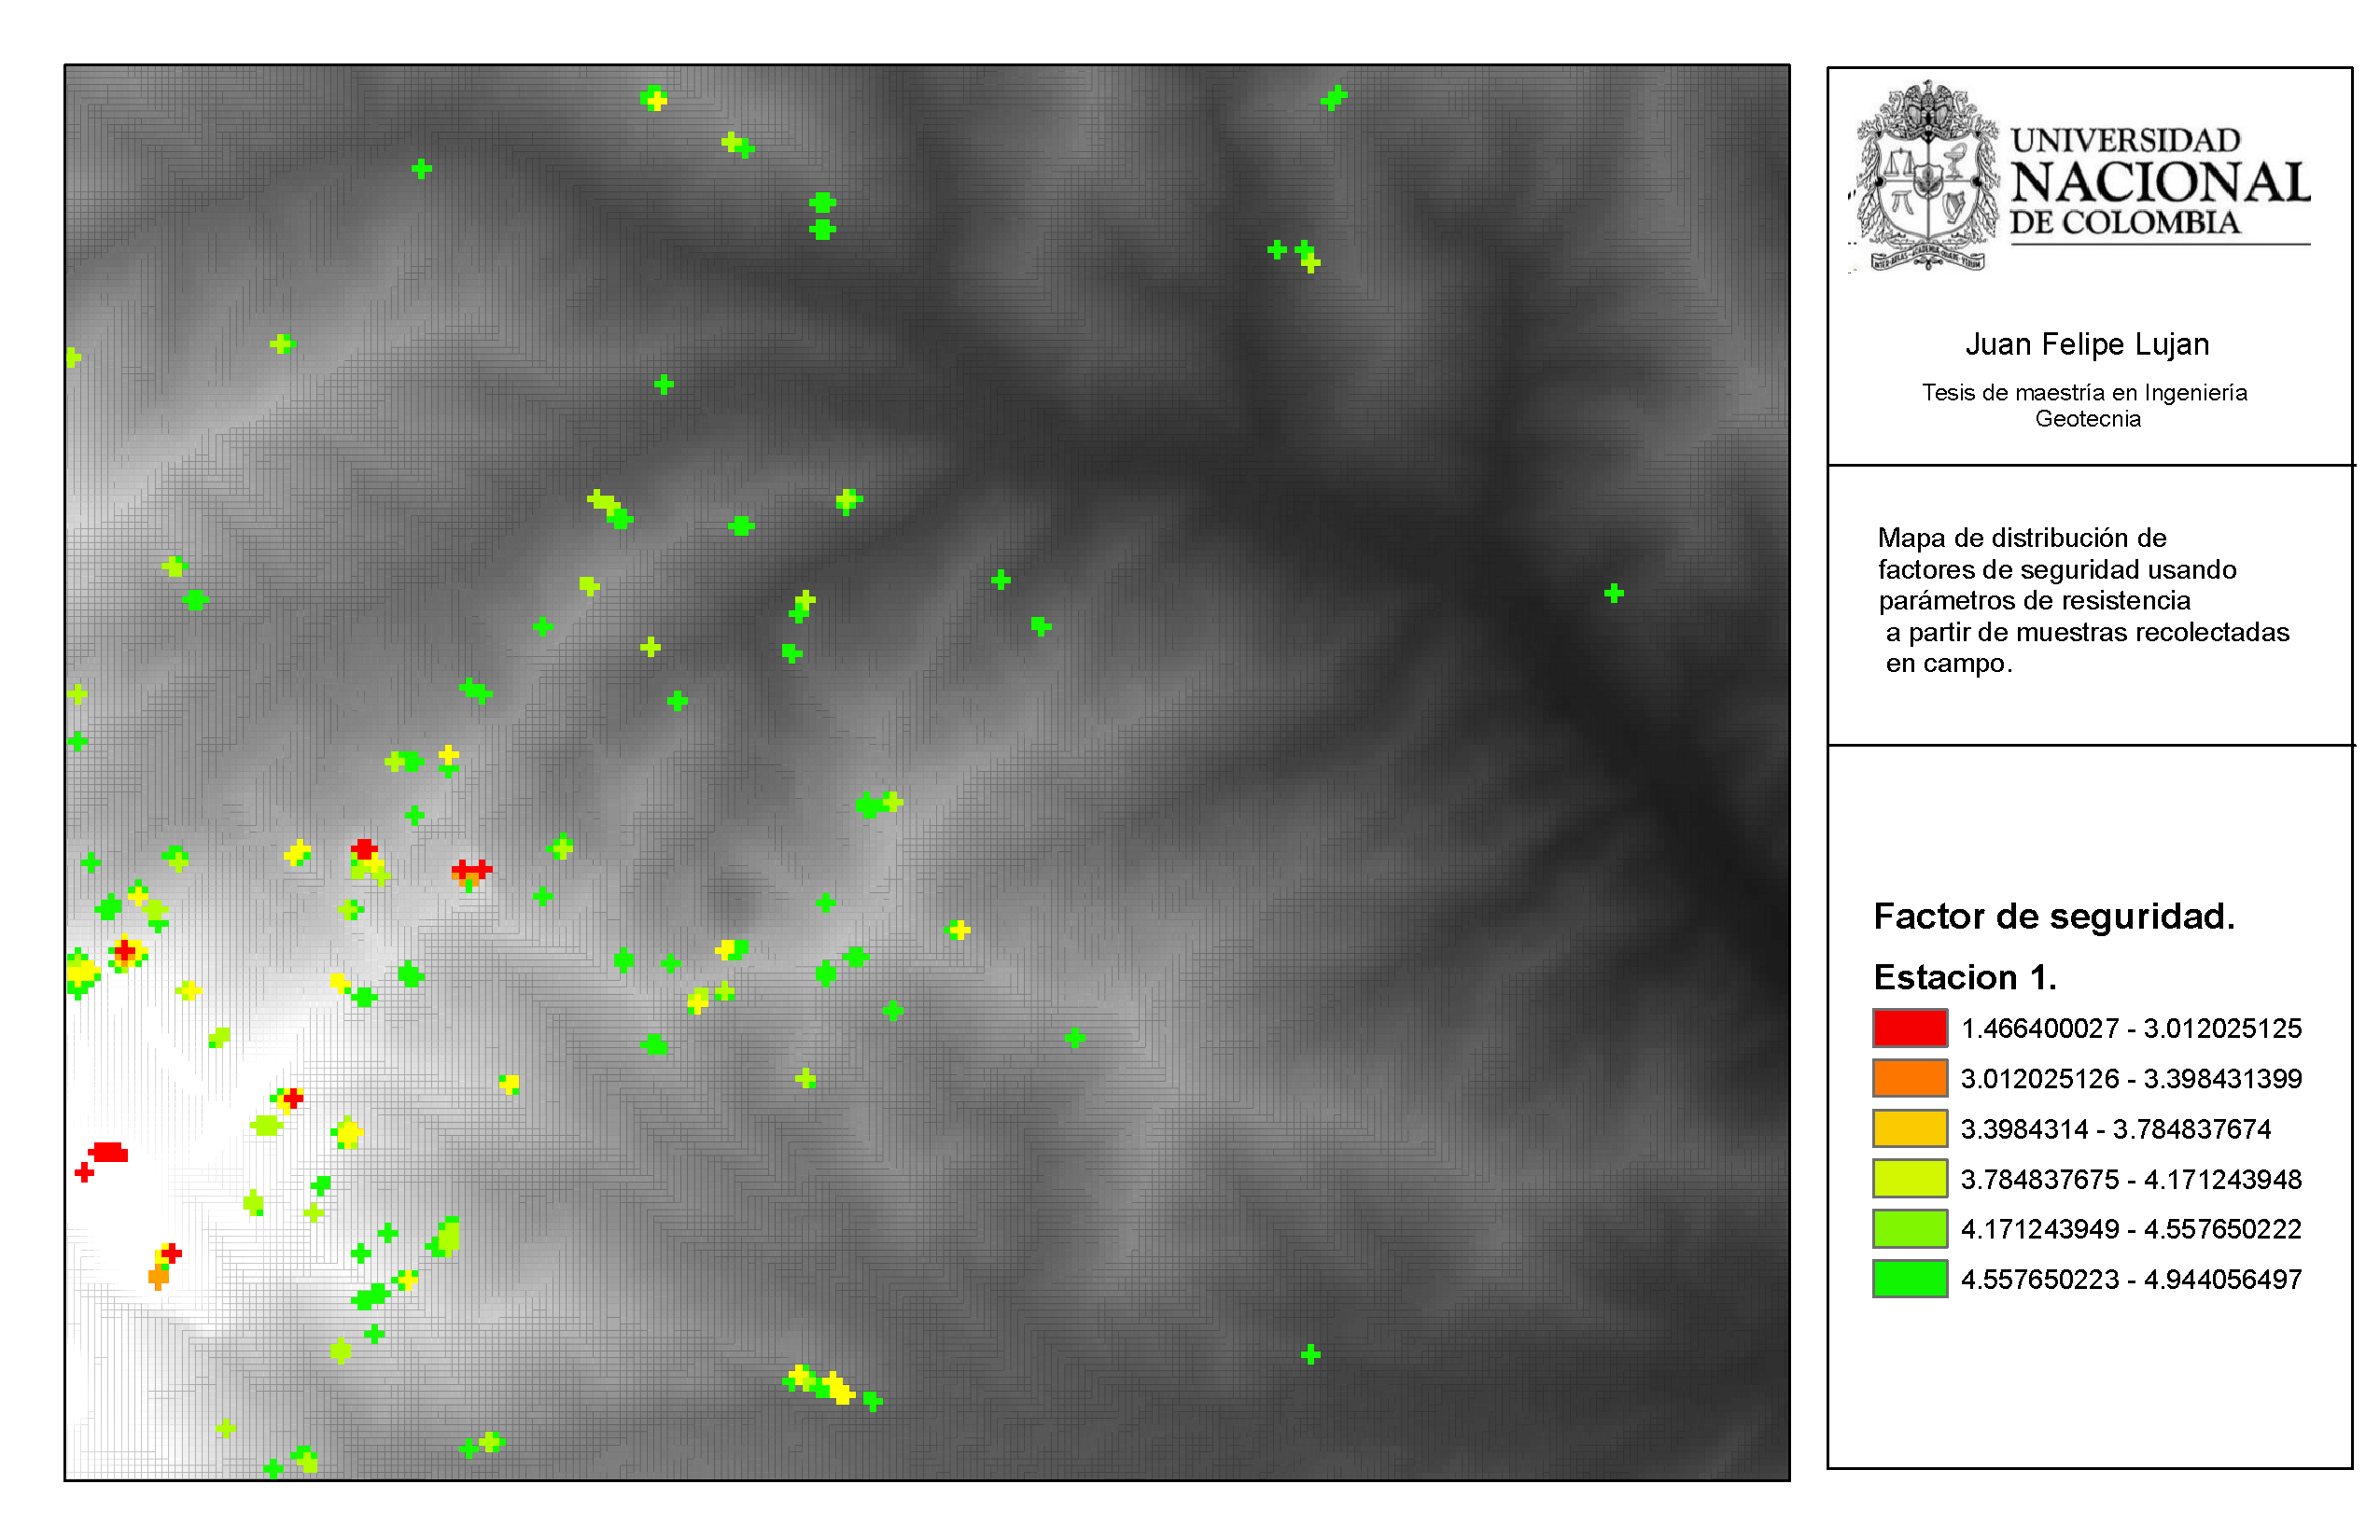
\includegraphics[scale=0.3]{img/fos3DCampo_coarse.pdf}
\caption{Resolutado inicial de la ejecici\'on de Scoops 3D usando la configuraci\'on usada en las pruebas preliminares (caja de busqueda).}
\label{fig:fos3dout_coarse}
\end{figure}

Inicialmente se realiz\'o una primera corrida de Scoops3D manteniendo la configuraci\'on de caja de b\'usqueda usada en las pruebas preliminares. Sin embargo, se encontr\'o que debido a la baja resoluci\'on, se presentaron extensas zonas del DEM que estaban excluidas del analis\'is, lo anterior porque algunas esferas de falla intersectaban el DEM en mas de 10 partes,  produciendo un mapa de distribuciones bastante imcompleto \ref{fig:fos3dout_coarse}. Aunque dicho comportamiento sea de esperarse durante la ejecici\'on de Scoops3D, una alta ocurrencia de sectores omitidos indica que la calidad del DEM usado no es \'optima.

Para reducir dicho efecto, se deshabilito la busqueda "de grueso a fino" (coarse to fine). Lo cual aumenta considerablemente el tiempo de ejecici\'on requerido por Scoops3D, debido a que no se realizan analisis con esferas de gran tamano, las cuales generaban una mayor cantidad de intersecciones, y por tal motivo estaban siendo omitidas.
Una vez realizado este cambio se pudo obtener el mapa de distribuciones ilustrado en la figura \ref{fig:fos3dout}.

\begin{figure}[H]
\centering
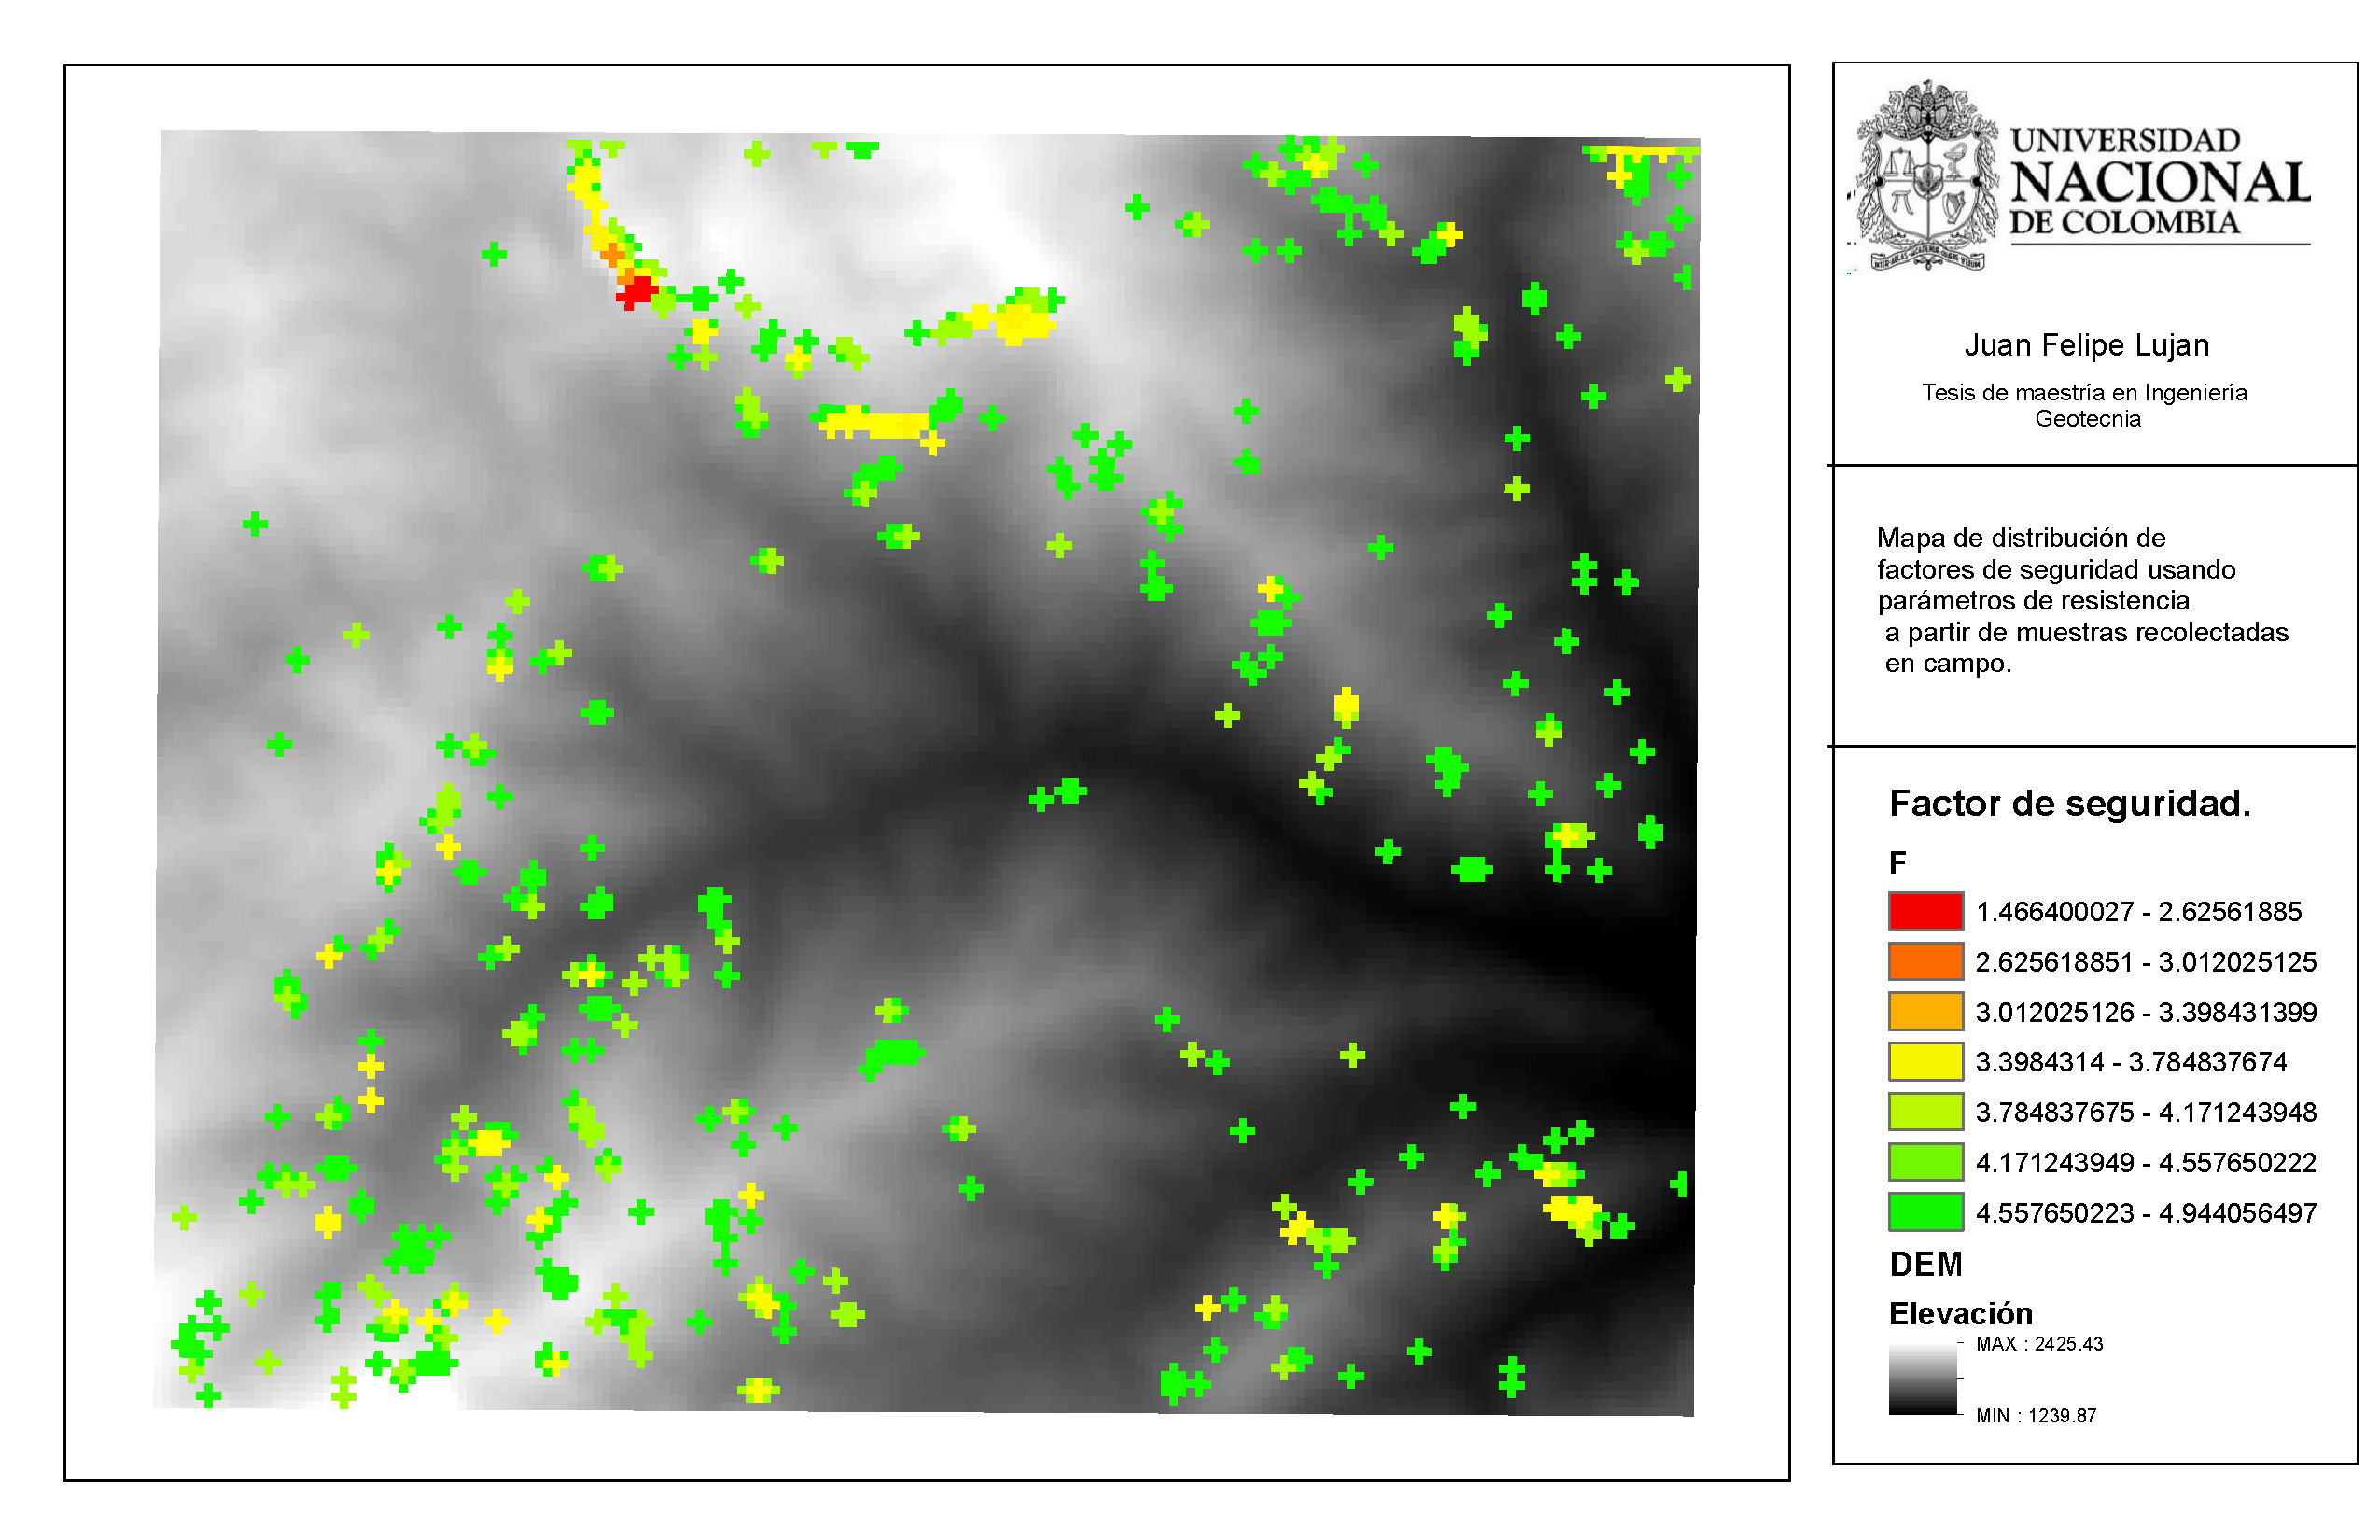
\includegraphics[scale=0.3]{img/fos3DCampo2.pdf}
\caption{Mapa de distribuci\'on de factores de seguridad en la zona de trabajo seg\'un el an\'alisis realizado con scoops 3D y muestras de la zona. Fuente: Elaboraci\'on propia.}
\label{fig:fos3dout}
\end{figure}

Como resultado del an\'alisis probabil\'istico por medio del m\'etodo Bishop utilizando las valores de resistencia obtenidos en los an\'alisis de laboratorio realizadas a las muestras recolectadas del \'area de trabajo se obtiene el mapa de \emph{distribuciones de factores de seguridad} presentado en la figura \ref{fig:fos3dout}.
Se analizaron un total de \(285\,744\) superficies de falla.

Como es de esperarse, los valores de factor de seguridad m\'as bajos se presentan hacia el suroccidente de la zona de trabajo, donde  son abundantes laderas con pendientes  largas y pronunciadas. All\'i los valores de factor de seguridad obtenidos de alcanzan \(1.46\) en cercan\'ias al Batolito Farallones y su aureola de contacto. 

Si se considera un \textit{cutoff} de 3.0 para el factor de seguridad, el cuerpo de masa de mayores dimensiones con factor de seguridad  inferior a dicho \textit{cutoff} ($2.43$ espec\'ificamente) posee una masa de $9.544\,\text{kg}$, in vol\'umen de 231.34 m3 y se extiende sobre 23.63 m3



\section{Conclusiones}


Aunque se han encontrado zonas espec\'ificas con factor de seguridad bajo, estas abarcan pocas extensiones (poca superficie) y poco distribuidas, no se han detectado zonas de embergadura considerable con \textit{F} inferior a 3.0.

La informaci\'on de cohesion, \'angulo de fricci\'on y peso especif\'ico tradicionalmente usado en Bishop simplificado para dos dimensiones puede usarse como insumo para extender el an\'alisis  de equilibrio l\'imite a 3D dimensiones.

La calidad del producto generado por Scoops3D se ve altamente beneficiada por el uso de informaci\'on SIG de alto nivel de detalle, toda vez que reduce la aparici\'on de multiples subsets por esfera de b\'usqueda. 





\section{Recomendaciones}

Previo al uso de la herramienta Scoops3D se recomienda en realizar un proceso de control de calidad sobre el DEM utilizado. Con el proposito de extraer los metadatos de extension horizontal y veltical del mismo para el momento de asignar las dimensiones a la caja de busqueda en Scoops3D.

Realizar un recorte (crop) al dem para evaluar en Scoops3D \'unicamente en la zona requerida, esto para reducir el timepo de ejecuci\'on de Scoops3D

Seleccionar siempre la opci\'on de Bishop dentro del menu de selecci\'on de an\'alisis de estabilidad, ya que esta opcio\'n calcula el factor de seguridad tanto por Bishop simplificado como por el m\'etodo de Fellenius.

Siempre realizar corridas de prueba en Scoops3D con par\'ametros de resistencia estimados, para evaluar la optima configuraci\'on de Scoops3D, espec\'ificamente para verificar que la caja de b\'usqueda no sea una limitante al momento de evaluar los m\'etodos bishop y fellenius al DEM usado.

Al utitlizar modelos de elevaci\'on digital de alta resoluci\'on ($5m^{2}$ o inferior tama\~no de pixel) es aconsejable usar servicios de computaci\'on en la nube como Google Cloud Platform (GCP) o Amazon Web Services (AWS) y la l\'inea de comando (CLI) en Python. Esto para acelerar los tiempos de ejecuci\'on
de Scoops3D